\chapter{Teorija}

U poglavlju nakon uvodnog uobičajeno se detaljnije opisuje
metodologija koja će se primijeniti u rješavanju završnog zadatka/diplomskog
rada, itd. Dakle navodi se opis primijenjenog modela, teorije, razrada
konstrukcijskog zadatka i sl.

\section{Opis modela}
Slijedi opis modela, teoretskog, matematičkog, eksperimentalnog ili koji je već
primijenjen u radu. Primjerice, model razmatran u radu prikazan je
relacijom~\eqref{eq:model}
\begin{equation}\label{eq:model}
\sum\limits_{k = 1}^m {\left( {\sin n\theta_j + n\frac{c_j a_{0j}}{2} \frac{\sin n\theta_j}
{\sin \theta_j}} \right)} \cdot A_k = \frac{c_j a_{0j}}{2} \left( {\alpha + \Delta\alpha_j - \alpha_{0j} } \right)\:,\quad j = 1,2,\ldots,m\:,
\end{equation} 
\nomenclature[gal]{$\alpha$}{napadni kut, [rad]}%
\nomenclature[galn]{$\alpha_0$}{napadni kut nultog uzgona profila, [rad]}%
\nomenclature[gda]{$\Delta\alpha$}{geometrijski kut uvijanja krila na promatranom rasponu, [rad]}%
\nomenclature[ec]{$c$}{duljina tetive krila, [m]}%
\nomenclature[eb]{$b$}{raspon krila, [m]}%
\nomenclature[gth]{$\theta$}{Glauertova varijabla za raspon, [rad]}%
\nomenclature[ean]{$a_0$}{gradijent koeficijenta sile uzgona po napadnom kutu}%
\nomenclature[ij]{$j$}{$j$--ti presjek na rasponu krila}%
\nomenclature[aa]{$A_k$}{koeficijenti Fourierovog reda}%
uz $n = 2k - 1$. Traženo rješenje za intenzitet cirkulacije $\Gamma_j$ na
promatranom rasponu $j$ je
\begin{equation} 
\frac{\Gamma_j}{{2b\Vinf}} = \sum_{k=1}^{m}{A_k\sin{n\theta_j}}\:,\quad n=2k-1\:.
\end{equation} 
\nomenclature[iinf]{$\infty$}{značajke neporemećene struje}%
\nomenclature[av]{$\Vinf$}{brzina neporemećene struje, [m/s]}%
\nomenclature[gg]{$\Gamma$}{intenzitet cirkulacije, [$\rm m^2/\rm s$]}%

\section{Detalji modela}
Poželjno je koristiti i slike, kada to može doprinijeti preglednosti i uvidu u model (kao
npr. slika~\ref{fig:model}). 
%
\begin{figure}[H]
	\centering
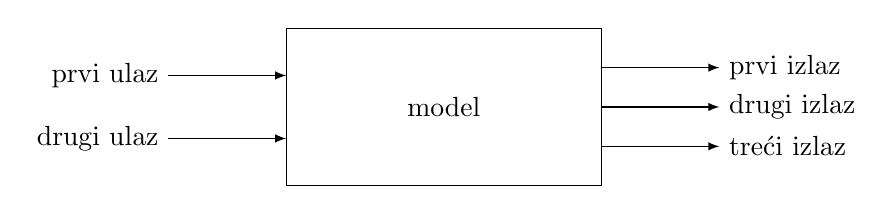
\begin{tikzpicture}
	\draw (0,0) rectangle (4,2);
	\draw (2,1) node[text width=3cm, text badly centered]{model};
	\draw[latex-] (0,0.6)--(-1.5,0.6) node[left] {drugi ulaz};
	\draw[latex-] (0,1.4)--(-1.5,1.4) node[left] {prvi ulaz};
	\draw[-latex] (4,0.5)--(5.5,0.5) node[right] {treći izlaz};
	\draw[-latex] (4,1)--(5.5,1) node[right] {drugi izlaz};
	\draw[-latex] (4,1.5)--(5.5,1.5) node[right] {prvi izlaz};
\end{tikzpicture}
\caption{Shema modela; izrađena primjenom Ti\textit{k}Z paketa}
	\label{fig:model}
\end{figure}

Poželjno je sve slike koje se nalaze u radu pozvati u tekstu (kao ovdje na
sliku~\ref{fig:unizg}).
\begin{figure}[H]
  \centering
  
\includegraphics[height=3.2cm]{02_Teorija/unizg_sivi_t4s}\\
  \hangcaption{Primjer slike; UNIZG logo}
  \label{fig:unizg}
\end{figure}
\nomenclature[Ku]{UNIZG}{Sveučilište u Zagrebu}%

\subsection{Razrada}
Detaljnija razrada modela, metodologije, konstrukcijskog zadatka, kao npr.
modela \eqref{eq:model} mogu se opisati kao u
\eqref{eq:ls-1}
\begin{equation}\label{eq:ls-1}
	c_l(y)=\frac{2\Gamma(y)}{\Vinf\;c(y)}\:.
\end{equation}
\nomenclature[ecal]{$c_l$}{lokalni koeficijent uzgona\nomrefeq}%
Pri tome treba imati mjeru i ne prenositi u tekstu nepotrebne izvode,
ponavljanja iz udžbenika i sl.
